%=====================================================================
\section{Collateral-Aware Evaluation: Details}
\label{app:eval}
%=====================================================================

\subsection{Collateral Questions}
For every edited token with a common meaning outside the concept (e.g., \emph{Harry}, \emph{Caesar}, \emph{club}), LLM agents (Claude) wrote four-option multiple-choice questions that use the token in that meaning, and other agents reviewed them, both without knowing which methods would be scored.
Items that the unedited model answers incorrectly under either option order were dropped, and each split was frozen with a hash before any edited model was scored.
The held-out set has \expnum{3{,}501} items on \expnum{1{,}026} tokens.
Collateral accuracy is normalized against the unedited model per token, like \ember{}'s metrics.

\subsection{Scores, Gates and Selection Rules}
$\Hthree$ is the harmonic mean of efficacy, specificity and collateral; $H_4$ adds Alpaca coherence.
A point is admissible only if MMLU stays at or above 0.9 and validation collateral at or above 0.8 of the unedited model.
Each rule selects one grid point per run on validation and scores it once on test:

\begin{center}
\small
\setlength{\tabcolsep}{3pt}
\begin{tabular}{@{}lP{3.4cm}l@{}}
\toprule
Rule & Selects & Role \\
\midrule
Collateral & max $\Hthree$, both gates & primary \\
Paper & max $\hmean$(efficacy, specificity), MMLU gate & the old protocol \\
Fixed & the point $r = 0.5$ & equal edit size \\
Integrity & collateral rule, copy $\geq 0.9$ & words stay readable \\
\bottomrule
\end{tabular}
\end{center}

\subsection{Word Integrity Tests}
\begin{center}
\small
\setlength{\tabcolsep}{3pt}
\begin{tabular}{@{}lP{4.6cm}@{}}
\toprule
Test & Question asked \\
\midrule
Copy & Can the model repeat a sentence containing the word? \\
What is X? & Free answer, labelled blindly as knowing the concept (leak), knowing another meaning or not knowing (graceful), inventing a meaning (confabulation), or not registering the word (destruction) \\
Context & Is an unrelated MMLU question placed after a sentence with the word still answered? \\
Generation & Do 20 neutral prompts per concept that use the edited words keep their answer? \\
\bottomrule
\end{tabular}
\end{center}

\noindent Free-text answers were labelled by LLM agents that never saw which method produced them; 10\% of items were duplicated across agents, with agreement \expnum{0.92--0.97} on the exact label and \expnum{0.97--1.00} on the decisive class.
Each test is also run on the real word, the word deleted, and a nonce.
The \emph{nonce floor} and the \emph{deletion floor} are the efficacies of the unedited model on the concept questions with the edited words replaced by their nonces or deleted.

\subsection{Pre-registration and Robustness}
Analysis plans were written into a pre-registration and amendments, nearly all before their results existed (amendment 2, the intention-to-treat analysis and the McNemar test are exceptions).
The primary endpoint pairs only runs where both methods edit; Table~\ref{tab:robust} varies this and the collateral gate (all post hoc, defined after the primary result).

% Sources: results/varwidth/layers/collateral/confirm.md ("Primary" and "Sensitivity (amendment 9, post hoc)");
% Holm p of the gate rows: results/varwidth/layers/collateral/coverage_split.md ("both edit" columns).
\begin{table}[ht]
\centering
\footnotesize
\setlength{\tabcolsep}{2.5pt}
\begin{tabular}{@{}lcccc@{}}
\toprule
 & \multicolumn{4}{c}{$\Delta\Hthree$ vs.\ \ember{}} \\
\cmidrule(l){2-5}
Setting & \cinder{} & -RS & -z & -RS-z \\
\midrule
Primary & \expnum{$+.042$} & \expnum{$+.034$} & \expnum{$+.132$} & \expnum{$+.084$} \\
\quad Holm $p$ & \expnum{.41} & \expnum{.41} & \expnum{.074} & \expnum{.074} \\
All 60 runs & \expnum{$+.123$} & \expnum{$+.133$} & \expnum{$+.167$} & \expnum{$+.178$} \\
\quad Holm $p$ & \expnum{.10} & \expnum{.10} & \expnum{.10} & \expnum{.049} \\
Gate 0.9 & \expnum{$+.174$} & \expnum{$+.147$} & \expnum{$+.195$} & \expnum{$+.102$} \\
\quad Holm $p$ & \expnum{.012} & \expnum{.012} & \expnum{.008} & \expnum{.014} \\
Gate 0.7 & \expnum{$-.019$} & \expnum{$-.041$} & \expnum{$+.121$} & \expnum{$+.070$} \\
\quad Holm $p$ & \expnum{.73} & \expnum{.73} & \expnum{.27} & \expnum{.72} \\
Leave one out & \expnum{.03--.06} & \expnum{.01--.06} & \expnum{.11--.16} & \expnum{.06--.10} \\
\quad $p$ & \expnum{.08--.38} & \expnum{.16--.70} & \expnum{.004--.04} & \expnum{.004--.05} \\
\bottomrule
\end{tabular}
\caption{Robustness of the primary comparison (paired test $\Hthree$, unit = concept; 11 held-out concepts where both edit, 12 for all runs). Columns: \cinder{}, \cinder{}-RS, \cinderz{}, \cinder{}-RS-z. Primary: runs where both edit. All rows below it are post hoc. All 60 runs: a run without an edit is scored as the unedited model. Gate: the collateral rule rerun on the saved grids with the collateral gate at 0.9 or 0.7 instead of 0.8. Leave one out: range of the mean difference and of the uncorrected $p$ over the 11 omitted concepts.}
\label{tab:robust}
\end{table}

\paragraph{Development claims on held-out concepts}
The evaluation was developed on 3 concepts (Harry Potter, Ancient Rome, Valentine's Day; 8 concept-seeds) and then frozen.
Table~\ref{tab:devclaims} lists the development claims and what the 12 held-out concepts (60 runs) showed.
Of the eight claims, four replicate, one replicates only in part, and three do not; the development ordering of the variants, in particular, did not hold, so the main text compares methods only on held-out concepts.

% Sources: CINDER_collateral_evaluation.md, findings F1-F29 and F44 (development F1-F23, held out F24-F29, F44);
% numbers: results/varwidth/layers/collateral/{poc,confirm,twobytwo}.md.
\begin{table}[ht]
\centering
\footnotesize
\setlength{\tabcolsep}{3pt}
\begin{tabular}{@{}P{2.7cm}P{3.1cm}P{1.3cm}@{}}
\toprule
Development claim & Held-out result & Verdict \\
\midrule
Without collateral, selection picks destructive edits (\ember{} at $r = 10$--$100$ in \expnum{6 of 6} runs) & paper rule: \ember{} and \cinderz{} at median $r = \expnum{100}$; ours: every method at median $r = \expnum{1}$ & replicated \\
\addlinespace
At small $r$, \cinder{}'s direction removes more (efficacy \expnum{.33} vs.\ \expnum{.20} at $r = 0.5$, validation) & at $r = 0.5$, every variant beats \ember{} on \expnum{10 of 11} concepts (\cinder{} $\Delta\Hthree$ \expnum{$+.15$}, Holm $p$ \expnum{.012}) & replicated \\
\addlinespace
The gain is the direction, not the token set ($\Delta_{\text{dir}}$ efficacy \expnum{$+.15$} at $r = 0.25$, \expnum{$+.09$} at $r = 1$; 5 runs) & \expnum{$+.07$} at $r = 0.5$ (\expnum{10 of 11}, Holm $p$ \expnum{.097}); \expnum{$-.02$} at $r = 1$ & at $r = 0.5$ only \\
\addlinespace
At their own operating points the methods tie (test $\Hthree$ \expnum{.42} vs.\ \expnum{.42}) & \cinder{} \expnum{$+.04$}, Holm $p$ \expnum{.41} & replicated \\
\addlinespace
\cinder{}-RS is the strongest variant ($\Hthree$ \expnum{.46}) & \cinder{}-RS \expnum{$+.03$}; the -z variants lead (\expnum{$+.13$}, \expnum{$+.08$}) & not replicated \\
\addlinespace
The original-space edit (-z) does not help (\expnum{$-.01$} and \expnum{$-.06$} vs.\ its parent) & \cinderz{} \expnum{$+.13$} vs.\ \ember{} (\expnum{9 of 11}, Holm $p$ \expnum{.074}) & not replicated \\
\addlinespace
\cinder{} destroys fewer words (destruction \expnum{.21} vs.\ \expnum{.30}; exclusive words \expnum{.37} vs.\ \expnum{.74}) & \expnum{.52} vs.\ \expnum{.49}; exclusive \expnum{.70} vs.\ \expnum{.65} (n.s.) & not replicated \\
\addlinespace
Under the paper's rule \ember{} beats \cinder{}, and the -z edit reaches \ember{} by deleting the words & \cinder{} wins \expnum{1 of 11} concepts on $H_2$; \cinderz{} wins \expnum{11 of 11} at $r = \expnum{100}$ & replicated \\
\bottomrule
\end{tabular}
\caption{Development claims (3 concepts, 2--3 seeds) and their held-out test (12 concepts, 5 seeds, test split). Differences are paired against \ember{} on runs where both edit, unless stated otherwise.}
\label{tab:devclaims}
\end{table}

\paragraph{Mean and Noise (development only)}
Following \ember{}, Mean replaces each edited embedding by the vocabulary mean and Noise subtracts a random direction of the same length; both use the edited tokens of \ember{} or \cinder{} and the same grid, gates and selection (Table~\ref{tab:baselines}).
Mean has a single point ($r \approx \expnum{0.85}$--$\expnum{0.95}$), whose validation collateral is \expnum{0.71} (\expnum{0.55}--\expnum{0.78}), so it fails the collateral gate in every run and is never selected; at that point it deletes the words (3 labelled runs: copy \expnum{0}, destruction \expnum{0.99}) while the rest of the prompt is still read (context accuracy \expnum{0.52}--\expnum{0.54}).
Noise at its selected points (median $r = 1$; same 3 runs) destroys \expnum{0.25}--\expnum{0.35} of the edited words and still leaks the concept in \expnum{0.29} of the free answers.
We did not run the baselines on the held-out concepts.

% Source: results/varwidth/layers/collateral/poc.md ("Mean over concept-seeds"); Mean's point and the integrity numbers:
% CINDER_collateral_evaluation.md F7, F12, F15 (T3 labels on 3 runs).
\begin{table}[ht]
\centering
\footnotesize
\setlength{\tabcolsep}{3.5pt}
\begin{tabular}{@{}lccccc@{}}
\toprule
Method (tokens) & Runs & Eff. & Coll. & $\Hthree$ & mean $r$ \\
\midrule
\ember{} & \expnum{6} & \expnum{.22} & \expnum{.93} & \expnum{.42} & \expnum{0.76} \\
\quad Noise (\ember{}'s) & \expnum{6} & \expnum{.22} & \expnum{.91} & \expnum{.40} & \expnum{1.09} \\
\quad Mean (\ember{}'s) & \expnum{6} & \multicolumn{4}{c}{no admissible point} \\
\cinder{} & \expnum{7} & \expnum{.21} & \expnum{.87} & \expnum{.42} & \expnum{1.71} \\
\quad Noise (\cinder{}'s) & \expnum{7} & \expnum{.18} & \expnum{.89} & \expnum{.34} & \expnum{1.57} \\
\quad Mean (\cinder{}'s) & \expnum{7} & \multicolumn{4}{c}{no admissible point} \\
\bottomrule
\end{tabular}
\caption{Embedding-editing baselines on the development concepts (test split, collateral rule; mean over concept-seeds). A run without an admissible point is not edited.}
\label{tab:baselines}
\end{table}

\subsection{Integrity-Gated Selection}

\begin{figure}[t]
  \centering
  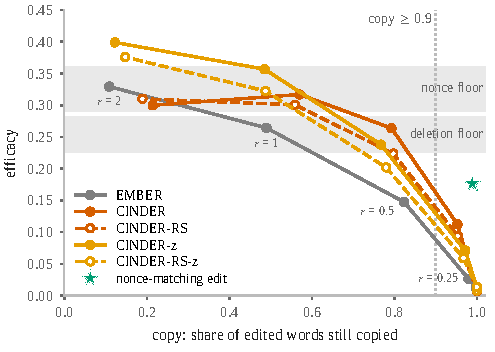
\includegraphics[width=\columnwidth]{figures/integrity.pdf}
  \caption{Removing more costs the words. Mean efficacy against the share of edited words the model can still copy, along the edit-size grid $r = 0.05, \dots, 2$ (labelled on \ember{}'s curve), over the held-out runs where each method edits (\expnum{41}--\expnum{55} of 60; validation questions). Grey bands: the efficacy of the unedited model when the edited words are replaced by their nonces (nonce floor, \expnum{0.29}--\expnum{0.36}) or deleted (deletion floor, \expnum{0.23}--\expnum{0.28}) in the test questions, over the five methods' token sets; dotted line: the integrity gate (copy $\geq 0.9$). Every method crosses its (test) deletion floor between $r = 0.5$ and $1$, where copy falls from about \expnum{0.8} to \expnum{0.5}, and none reaches its nonce floor while more than half of its words remain copyable. Star: the free nonce-matching edit on \cinder{}'s tokens (post hoc; seed 42, \expnum{9} runs, test split), which keeps \expnum{0.99} of the words copyable at efficacy \expnum{0.18}.}
  \label{fig:integrity}
\end{figure}
Figure~\ref{fig:integrity} shows the trade-off that this rule cuts through.
The integrity-gated rule (post hoc) is the collateral rule restricted to grid points where at least 90\% of the edited words can still be copied; the copy test was run at every grid point up to $r = 2$ (\expnum{1{,}530} points).
It coincides with the collateral-rule point in only \expnum{16} of \expnum{255} run-variants.
Table~\ref{tab:e3} gives the result.
On the paired endpoint of the primary analysis (runs where both edit), \cinder{} gains \expnum{$+0.096$} $\Hthree$ over \ember{} (95\% CI \expnum{$[-0.006, +0.214]$}, \expnum{7}--\expnum{3} concepts, Holm $p = \expnum{0.42}$) and \cinder{}-RS \expnum{$+0.092$} (\expnum{7}--\expnum{3}, \expnum{0.42}), the -z variants \expnum{$+0.029$} and \expnum{$+0.026$} (\expnum{0.75}).
Counting runs without an edit as no erasure, \cinder{} gains \expnum{$+0.134$} (\expnum{10}--\expnum{2}, Holm $p = \expnum{0.015}$) and \cinder{}-RS \expnum{$+0.166$} (\expnum{11}--\expnum{1}, \expnum{0.006}), the -z variants \expnum{$+0.053$} and \expnum{$+0.063$} (\expnum{0.33}).
The -z edits break copying at smaller $r$, so the rule pushes them to $r = 0.05$ in \expnum{24 of 52} and \expnum{26 of 55} runs.
Alpaca coherence at these points (seed 42) is \expnum{0.97--0.98} for every method.

% Source: results/varwidth/layers/collateral/last_mile.md ("E3: integrity-gated selection"); H4: last_mile.md Alpaca table,
% point e3 (seed 42); all-runs contrasts: coverage_split.md ("Integrity-gated"); r = 0.05 counts and 16/255:
% CINDER_collateral_evaluation.md F38.
\begin{table}[ht]
\centering
\footnotesize
\setlength{\tabcolsep}{2.4pt}
\begin{tabular}{@{}lccccccc@{}}
\toprule
Method & Runs & Eff. & Coll. & $\Hthree$ & $r$ & \shortstack{Copy\\ex./mu.} & $H_4$ \\
\midrule
\ember{} & \expnum{41} & \expnum{.06} & \expnum{.98} & \expnum{.12} & \expnum{0.1} & \expnum{.98/.99} & \expnum{.18} \\
\cinder{} & \expnum{52} & \expnum{.12} & \expnum{.97} & \expnum{.25} & \expnum{0.25} & \expnum{.96/.97} & \expnum{.35} \\
\cinder{}-RS & \expnum{55} & \expnum{.14} & \expnum{.98} & \expnum{.27} & \expnum{0.25} & \expnum{.94/.97} & \expnum{.20} \\
\cinderz{} & \expnum{52} & \expnum{.07} & \expnum{.99} & \expnum{.16} & \expnum{0.25} & \expnum{.97/.99} & \expnum{.16} \\
\cinder{}-RS-z & \expnum{55} & \expnum{.07} & \expnum{.99} & \expnum{.16} & \expnum{0.1} & \expnum{.98/.98} & \expnum{.25} \\
\bottomrule
\end{tabular}
\caption{Integrity-gated selection (copy $\geq 0.9$; post hoc) on the 12 held-out concepts, test split. Runs: runs with an edit (of 60); means over those runs; $r$: median edit size; copy for concept-exclusive and multi-meaning words separately; $H_4$ adds Alpaca coherence (seed 42 only, 8--10 runs).}
\label{tab:e3}
\end{table}

\subsection{Direction or Token Set}
\label{app:dir}

\begin{figure}[t]
  \centering
  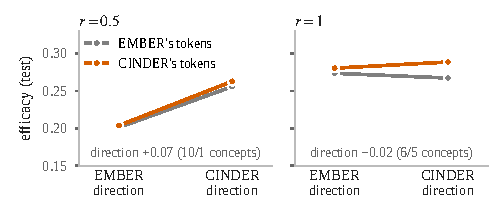
\includegraphics[width=\columnwidth]{figures/twobytwo.pdf}
  \caption{Test efficacy of the four direction $\times$ token-set cells (post hoc). At $r = 0.5$, switching to \cinder{}'s direction adds \expnum{$+0.07$} (\expnum{10 of 11} concepts) and switching to \cinder{}'s tokens \expnum{$+0.02$}, so the two lines nearly coincide; at $r = 1$ the direction effect vanishes (\expnum{$-0.02$}, \expnum{6}/\expnum{5} concepts). \ember{}'s own cell averages its 41 runs, the other cells 38.}
  \label{fig:twobytwo}
\end{figure}
Four cells cross the token set with the direction at a fixed $r = 0.5$, on the runs where \ember{} has a token set; ``\cinder{}'s tokens'' are \cinder{}'s top concept-only tokens, as many as \ember{} edits.
All cells use dense coefficients so that every token has a coefficient on $\Fc$.

\begin{center}
\small
\setlength{\tabcolsep}{4pt}
\begin{tabular}{@{}lcc@{}}
\toprule
Efficacy / $\Hthree$ & \ember{} direction & \cinder{} direction \\
\midrule
\ember{} tokens & \expnum{.20 / .39} & \expnum{.26 / .46} \\
\cinder{} tokens & \expnum{.20 / .39} & \expnum{.26 / .48} \\
\bottomrule
\end{tabular}
\end{center}

\noindent The direction effect (mean of the row differences) is \expnum{$+0.073$} efficacy and \expnum{$+0.097$} $\Hthree$, on \expnum{10 of 11} concepts (Holm $p$ \expnum{0.097} and \expnum{0.055}); the token-set effect is \expnum{$+0.016$} and \expnum{$+0.024$} (n.s.); the direction costs \expnum{0.02} collateral.
At $r = 1$ (secondary), the cell means are \expnum{.27 / .47} (\ember{} tokens, \ember{} direction), \expnum{.27 / .45} (\ember{} tokens, \cinder{} direction), \expnum{.28 / .46} (\cinder{} tokens, \ember{} direction) and \expnum{.29 / .48} (\cinder{} tokens, \cinder{} direction); the direction effect is \expnum{$-0.016$} efficacy ($p = \expnum{0.97}$) and \expnum{$-0.007$} $\Hthree$ ($p = \expnum{1.0}$), and the token-set effect \expnum{$+0.010$} and \expnum{$+0.012$} (both n.s.).

\subsection{The Nonce-Matching Edit}
\label{app:nonce}
We keep the model frozen and learn a change to each edited row.
The loss pushes the edited model, on concept sentences and new definitional prompts, toward what the unedited model does when the word is replaced by its nonce, while two further terms keep the word copyable (new carrier sentences) and keep the other meanings of multi-meaning tokens (sentences the model generated itself); no evaluation item is used for training.
The edit is either confined to the span of the edit set's concept components (rank $\leq 3$) or free, and is learned on \cinder{}'s or \ember{}'s token set; one free variant also adds concept questions that the model wrote itself to the forget data (+QA).
Selection is the integrity-gated rule; a run reaches the \emph{nonce point} when its test efficacy is at least its nonce floor minus 0.05, with copy $\geq 0.9$ and collateral $\geq 0.8$ (all post hoc, seed 42; Table~\ref{tab:nonce}).
The nonce floor averages \expnum{0.36} on the runs with \cinder{}'s tokens and \expnum{0.26}--\expnum{0.27} on those with \ember{}'s, and almost all runs that reach the nonce point have a floor near 0 (COVID-19 \expnum{0.00}, Pornography \expnum{0.07}--\expnum{0.11}); only Baseball (free, \ember{}'s tokens: \expnum{0.36} vs.\ floor \expnum{0.31}) and Heroin (+QA: \expnum{0.44} vs.\ \expnum{0.49}) reach a substantial floor.
Free edits move the rows far (median $r = \expnum{3}$, \expnum{3.2} and \expnum{1.6}) and keep them copyable, and remove \expnum{2--3$\times$} as much as integrity-gated \ember{} and \expnum{1.3--1.6$\times$} as much as integrity-gated \cinder{} on the same runs; paired $\Hthree$ against it (uncorrected): free (\cinder{}'s tokens) $-$ \cinderz{} \expnum{$+0.20$} (\expnum{7 of 9} concepts, $p = \expnum{0.055}$), +QA $-$ \cinderz{} \expnum{$+0.26$} (\expnum{7}--\expnum{1}, $p = \expnum{0.039}$), free (\ember{}'s tokens) $-$ \ember{} \expnum{$+0.28$} (\expnum{6}--\expnum{1}, $p = \expnum{0.047}$).
But asked ``What is X?'', the free edits repeat the word in only \expnum{0.34}--\expnum{0.49} of the answers (unedited word \expnum{0.96}, nonce \expnum{0.75}) and name a different invented string in \expnum{32}--\expnum{47\%} (nonce \expnum{17\%}), which the blind labels count as destruction.
Inside the concept subspace the words stay intact but almost nothing is removed, and the concept still leaks in \expnum{0.39} (\cinder{}) and \expnum{0.53} (\ember{}) of the answers.

% Source: results/varwidth/layers/collateral/nonce_edit.md (variants table; E3 baselines on the same runs; T3 labels;
% generation damage; renamed rate); attainment details: CINDER_collateral_evaluation.md F39-F43.
\begin{table}[ht]
\centering
\footnotesize
\setlength{\tabcolsep}{2.2pt}
\begin{tabular}{@{}lcccccc@{}}
\toprule
Edit (tokens) & \shortstack{Nonce\\point} & Eff. & Coll. & Copy & Destr. & Broken \\
\midrule
\multicolumn{7}{@{}l}{\emph{Learned, inside the concept subspace}} \\
\quad \cinder{}'s & \expnum{1/10} & \expnum{.04} & \expnum{.99} & \expnum{.99} & \expnum{.01} & \expnum{.02} \\
\quad \ember{}'s & \expnum{2/8} & \expnum{.02} & \expnum{.96} & \expnum{.97} & \expnum{.04} & \expnum{.04} \\
\multicolumn{7}{@{}l}{\emph{Learned, free}} \\
\quad \cinder{}'s & \expnum{2/9} & \expnum{.18} & \expnum{.86} & \expnum{.99} & \expnum{.50} & \expnum{.16} \\
\quad \ember{}'s & \expnum{3/7} & \expnum{.21} & \expnum{.86} & \expnum{.99} & \expnum{.59} & \expnum{.15} \\
\quad \cinder{}'s +QA & \expnum{3/10} & \expnum{.22} & \expnum{.89} & \expnum{1.00} & \expnum{.47} & \expnum{.15} \\
\midrule
\multicolumn{7}{@{}l}{\emph{Subtraction, integrity-gated (same runs)}} \\
\quad \ember{} & -- & \expnum{.07} & \expnum{.98} & -- & -- & -- \\
\quad \cinder{} & -- & \expnum{.14} & \expnum{.97} & -- & -- & -- \\
\quad \cinderz{} & -- & \expnum{.06} & \expnum{.99} & -- & -- & -- \\
\bottomrule
\end{tabular}
\caption{The nonce-matching edit (post hoc; seed 42, 12 held-out concepts, test split). Nonce point: runs that reach the nonce point, of the runs with an edit; Copy: share of edited words copied; Destr.: share of ``What is X?'' answers labelled as not registering the word; Broken: share of the 20 neutral prompts per concept whose answer breaks.}
\label{tab:nonce}
\end{table}
